% Long version (ARR long paper, 8 pages + unlimited references/limitations/appendix).
% Build: tectonic -X compile main.tex   (or `make paper` from the repository root)
% preprint.tex defines \PREPRINT to build the non-anonymous arXiv version from this file.
\documentclass[11pt]{article}
\ifdefined\PREPRINT\usepackage[preprint]{acl}\else\usepackage[review]{acl}\fi
\usepackage{times}
\usepackage{latexsym}
\usepackage[T1]{fontenc}
\usepackage[utf8]{inputenc}
\usepackage{microtype}
\usepackage{inconsolata}
\usepackage{graphicx}
\usepackage{booktabs}
\usepackage{amsmath}
\usepackage{amssymb}
\usepackage{xspace}
\usepackage{siunitx}
\sisetup{group-separator={,},group-minimum-digits=4}
% Generated by scripts/paper_numbers.py -- do not edit. Ledger: CLAIMS.md
\newcommand{\alphaHx}{0.561\xspace}
\newcommand{\alphaLoHx}{0.552\xspace}
\newcommand{\alphaHiHx}{0.571\xspace}
\newcommand{\rawHx}{0.789\xspace}
\newcommand{\itemsHx}{20,148\xspace}
\newcommand{\ratersHx}{253\xspace}
\newcommand{\acOneHx}{0.592\xspace}
\newcommand{\ceilLooHx}{0.789\xspace}
\newcommand{\ceilInHx}{0.894\xspace}
\newcommand{\marginOneHx}{31.7\xspace}
\newcommand{\alphaHxthree}{0.460\xspace}
\newcommand{\alphaLoHxthree}{0.452\xspace}
\newcommand{\alphaHiHxthree}{0.467\xspace}
\newcommand{\rawHxthree}{0.644\xspace}
\newcommand{\itemsHxthree}{20,148\xspace}
\newcommand{\ratersHxthree}{253\xspace}
\newcommand{\acOneHxthree}{0.469\xspace}
\newcommand{\ceilLooHxthree}{0.644\xspace}
\newcommand{\ceilInHxthree}{0.814\xspace}
\newcommand{\marginOneHxthree}{46.6\xspace}
\newcommand{\alphaMhs}{0.425\xspace}
\newcommand{\alphaLoMhs}{0.416\xspace}
\newcommand{\alphaHiMhs}{0.434\xspace}
\newcommand{\rawMhs}{0.775\xspace}
\newcommand{\itemsMhs}{29,488\xspace}
\newcommand{\ratersMhs}{7,909\xspace}
\newcommand{\acOneMhs}{0.634\xspace}
\newcommand{\ceilLooMhs}{0.781\xspace}
\newcommand{\ceilInMhs}{0.883\xspace}
\newcommand{\marginOneMhs}{13.0\xspace}
\newcommand{\alphaMhsthree}{0.363\xspace}
\newcommand{\alphaLoMhsthree}{0.356\xspace}
\newcommand{\alphaHiMhsthree}{0.370\xspace}
\newcommand{\rawMhsthree}{0.686\xspace}
\newcommand{\itemsMhsthree}{29,488\xspace}
\newcommand{\ratersMhsthree}{7,909\xspace}
\newcommand{\acOneMhsthree}{0.585\xspace}
\newcommand{\ceilLooMhsthree}{0.695\xspace}
\newcommand{\ceilInMhsthree}{0.835\xspace}
\newcommand{\marginOneMhsthree}{16.6\xspace}
\newcommand{\alphaWiki}{0.464\xspace}
\newcommand{\alphaLoWiki}{0.460\xspace}
\newcommand{\alphaHiWiki}{0.469\xspace}
\newcommand{\rawWiki}{0.867\xspace}
\newcommand{\itemsWiki}{159,686\xspace}
\newcommand{\ratersWiki}{4,301\xspace}
\newcommand{\acOneWiki}{0.823\xspace}
\newcommand{\ceilLooWiki}{0.895\xspace}
\newcommand{\ceilInWiki}{0.924\xspace}
\newcommand{\marginOneWiki}{9.7\xspace}
\newcommand{\alphaWikiord}{0.296\xspace}
\newcommand{\alphaLoWikiord}{0.293\xspace}
\newcommand{\alphaHiWikiord}{0.299\xspace}
\newcommand{\rawWikiord}{0.482\xspace}
\newcommand{\itemsWikiord}{159,686\xspace}
\newcommand{\ratersWikiord}{4,301\xspace}
\newcommand{\alphaDthree}{0.158\xspace}
\newcommand{\alphaLoDthree}{0.113\xspace}
\newcommand{\alphaHiDthree}{0.208\xspace}
\newcommand{\rawDthree}{0.623\xspace}
\newcommand{\itemsDthree}{350\xspace}
\newcommand{\ratersDthree}{123\xspace}
\newcommand{\acOneDthree}{0.317\xspace}
\newcommand{\ceilLooDthree}{0.661\xspace}
\newcommand{\ceilInDthree}{0.774\xspace}
\newcommand{\marginOneDthree}{37.7\xspace}
\newcommand{\alphaDnine}{0.154\xspace}
\newcommand{\alphaLoDnine}{0.124\xspace}
\newcommand{\alphaHiDnine}{0.183\xspace}
\newcommand{\rawDnine}{0.666\xspace}
\newcommand{\itemsDnine}{990\xspace}
\newcommand{\ratersDnine}{166\xspace}
\newcommand{\acOneDnine}{0.449\xspace}
\newcommand{\ceilLooDnine}{0.706\xspace}
\newcommand{\ceilInDnine}{0.801\xspace}
\newcommand{\marginOneDnine}{31.8\xspace}
\newcommand{\alphaDthreethree}{0.149\xspace}
\newcommand{\alphaLoDthreethree}{0.108\xspace}
\newcommand{\alphaHiDthreethree}{0.190\xspace}
\newcommand{\rawDthreethree}{0.556\xspace}
\newcommand{\itemsDthreethree}{350\xspace}
\newcommand{\ratersDthreethree}{123\xspace}
\newcommand{\acOneDthreethree}{0.400\xspace}
\newcommand{\ceilLooDthreethree}{0.613\xspace}
\newcommand{\ceilInDthreethree}{0.729\xspace}
\newcommand{\marginOneDthreethree}{27.7\xspace}
\newcommand{\alphaMhsAll}{0.537\xspace}
\newcommand{\alphaMhsthreeAll}{0.470\xspace}
\newcommand{\alphaGoMedian}{0.230\xspace}
\newcommand{\alphaGoMin}{0.119\xspace}
\newcommand{\alphaGoMax}{0.715\xspace}
\newcommand{\goTopEmotion}{gratitude\xspace}
\newcommand{\nGoEmotions}{28\xspace}
\newcommand{\simFalseVoneIid}{0.08\xspace}
\newcommand{\simResVoneIid}{29.7\xspace}
\newcommand{\simFalseVtwoIid}{0.26\xspace}
\newcommand{\simResVtwoIid}{52.8\xspace}
\newcommand{\simFalseZlowIid}{1.29\xspace}
\newcommand{\simResZlowIid}{66.1\xspace}
\newcommand{\simFalseZmidIid}{0.26\xspace}
\newcommand{\simResZmidIid}{53.2\xspace}
\newcommand{\simResMatchedIid}{45.4\xspace}
\newcommand{\simCellsIid}{2,160\xspace}
\newcommand{\simResVoneLowAlphaIid}{0.03\xspace}
\newcommand{\simResZlowLowAlphaIid}{60.5\xspace}
\newcommand{\simFalseVoneHet}{0.07\xspace}
\newcommand{\simResVoneHet}{37.7\xspace}
\newcommand{\simFalseVtwoHet}{0.17\xspace}
\newcommand{\simResVtwoHet}{50.9\xspace}
\newcommand{\simFalseZlowHet}{0.92\xspace}
\newcommand{\simResZlowHet}{64.0\xspace}
\newcommand{\simFalseZmidHet}{0.17\xspace}
\newcommand{\simResZmidHet}{51.1\xspace}
\newcommand{\simResMatchedHet}{45.9\xspace}
\newcommand{\simCellsHet}{1,620\xspace}
\newcommand{\simResVoneLowAlphaHet}{0.03\xspace}
\newcommand{\simResZlowLowAlphaHet}{51.0\xspace}
\newcommand{\simFalseVoneHetneg}{0.43\xspace}
\newcommand{\simResVoneHetneg}{41.8\xspace}
\newcommand{\simFalseVtwoHetneg}{1.93\xspace}
\newcommand{\simResVtwoHetneg}{55.7\xspace}
\newcommand{\simFalseZlowHetneg}{5.47\xspace}
\newcommand{\simResZlowHetneg}{72.9\xspace}
\newcommand{\simFalseZmidHetneg}{2.24\xspace}
\newcommand{\simResZmidHetneg}{61.0\xspace}
\newcommand{\simResMatchedHetneg}{41.4\xspace}
\newcommand{\simCellsHetneg}{1,530\xspace}
\newcommand{\simResVoneLowAlphaHetneg}{0.09\xspace}
\newcommand{\simResZlowLowAlphaHetneg}{76.1\xspace}
\newcommand{\simFalseVoneHetmild}{0.16\xspace}
\newcommand{\simResVoneHetmild}{40.6\xspace}
\newcommand{\simFalseVtwoHetmild}{0.61\xspace}
\newcommand{\simResVtwoHetmild}{56.3\xspace}
\newcommand{\simFalseZlowHetmild}{2.43\xspace}
\newcommand{\simResZlowHetmild}{70.5\xspace}
\newcommand{\simFalseZmidHetmild}{0.63\xspace}
\newcommand{\simResZmidHetmild}{58.1\xspace}
\newcommand{\simResMatchedHetmild}{47.4\xspace}
\newcommand{\simCellsHetmild}{1,620\xspace}
\newcommand{\simResVoneLowAlphaHetmild}{0.08\xspace}
\newcommand{\simResZlowLowAlphaHetmild}{69.9\xspace}
\newcommand{\ablResRel}{48.8\xspace}
\newcommand{\ablResMde}{39.2\xspace}
\newcommand{\ablResCi}{29.7\xspace}
\newcommand{\ablResPrec}{29.7\xspace}
\newcommand{\ablResRepl}{29.7\xspace}
\newcommand{\ablResNone}{29.7\xspace}
\newcommand{\simComparisons}{2.16\xspace}
\newcommand{\clFourCells}{36\xspace}
\newcommand{\clFourWins}{36\xspace}
\newcommand{\clFourWikiKthree}{0.736\xspace}
\newcommand{\clFourWikiKthreePred}{0.831\xspace}
\newcommand{\clFourWikiKone}{0.989\xspace}
\newcommand{\clFourBelowPred}{78\xspace}
\newcommand{\clFourKgtOne}{108\xspace}
\newcommand{\clFourItemsWiki}{156,519\xspace}
\newcommand{\clFourEtaWiki}{0.071\xspace}
\newcommand{\clFourItemsDnine}{990\xspace}
\newcommand{\clFourEtaDnine}{0.202\xspace}
\newcommand{\clFourItemsDthree}{350\xspace}
\newcommand{\clFourEtaDthree}{0.239\xspace}
\newcommand{\retroN}{1,924\xspace}
\newcommand{\retroPairs}{15\xspace}
\newcommand{\retroUnresolvable}{4\xspace}
\newcommand{\retroBertGap}{0.008\xspace}
\newcommand{\retroBertPmax}{3.2\xspace}
\newcommand{\retroHuman}{76.9\xspace}
\newcommand{\retroSplit}{49.4\xspace}
\newcommand{\retroBestAcc}{0.698\xspace}
\newcommand{\allRatingsMaxShift}{0.022\xspace}
\newcommand{\mhsAnchorItems}{73\xspace}
\newcommand{\mhsAnchorShare}{32\xspace}
\newcommand{\attEstMaxErr}{0.003\xspace}
\newcommand{\retroMinGap}{0.002\xspace}
\newcommand{\retroMinPmax}{0.2\xspace}
\newcommand{\retroAlwaysGap}{0.061\xspace}
\newcommand{\jHumanHx}{0.872\xspace}
\newcommand{\jHumanLoHx}{0.847\xspace}
\newcommand{\jHumanHiHx}{0.896\xspace}
\newcommand{\jPanelItemsHx}{799\xspace}
\newcommand{\jHaikuHx}{0.777\xspace}
\newcommand{\jDiffHaikuHx}{-0.095\xspace}
\newcommand{\jDiffLoHaikuHx}{-0.129\xspace}
\newcommand{\jDiffHiHaikuHx}{-0.064\xspace}
\newcommand{\jGateHaikuHx}{BLOCK\xspace}
\newcommand{\jSonnetHx}{0.796\xspace}
\newcommand{\jDiffSonnetHx}{-0.077\xspace}
\newcommand{\jDiffLoSonnetHx}{-0.111\xspace}
\newcommand{\jDiffHiSonnetHx}{-0.044\xspace}
\newcommand{\jGateSonnetHx}{BLOCK\xspace}
\newcommand{\jGptHx}{0.757\xspace}
\newcommand{\jDiffGptHx}{-0.115\xspace}
\newcommand{\jDiffLoGptHx}{-0.151\xspace}
\newcommand{\jDiffHiGptHx}{-0.081\xspace}
\newcommand{\jGateGptHx}{BLOCK\xspace}
\newcommand{\jQwenHx}{0.675\xspace}
\newcommand{\jDiffQwenHx}{-0.198\xspace}
\newcommand{\jDiffLoQwenHx}{-0.235\xspace}
\newcommand{\jDiffHiQwenHx}{-0.156\xspace}
\newcommand{\jGateQwenHx}{BLOCK\xspace}
\newcommand{\jOssHx}{0.715\xspace}
\newcommand{\jDiffOssHx}{-0.158\xspace}
\newcommand{\jDiffLoOssHx}{-0.195\xspace}
\newcommand{\jDiffHiOssHx}{-0.121\xspace}
\newcommand{\jGateOssHx}{BLOCK\xspace}
\newcommand{\jHumanMhs}{0.803\xspace}
\newcommand{\jHumanLoMhs}{0.776\xspace}
\newcommand{\jHumanHiMhs}{0.829\xspace}
\newcommand{\jPanelItemsMhs}{863\xspace}
\newcommand{\jHaikuMhs}{0.803\xspace}
\newcommand{\jDiffHaikuMhs}{+0.000\xspace}
\newcommand{\jDiffLoHaikuMhs}{-0.030\xspace}
\newcommand{\jDiffHiHaikuMhs}{+0.031\xspace}
\newcommand{\jGateHaikuMhs}{BLOCK\xspace}
\newcommand{\jSonnetMhs}{0.788\xspace}
\newcommand{\jDiffSonnetMhs}{-0.015\xspace}
\newcommand{\jDiffLoSonnetMhs}{-0.048\xspace}
\newcommand{\jDiffHiSonnetMhs}{+0.017\xspace}
\newcommand{\jGateSonnetMhs}{BLOCK\xspace}
\newcommand{\jGptMhs}{0.765\xspace}
\newcommand{\jDiffGptMhs}{-0.038\xspace}
\newcommand{\jDiffLoGptMhs}{-0.072\xspace}
\newcommand{\jDiffHiGptMhs}{-0.006\xspace}
\newcommand{\jGateGptMhs}{BLOCK\xspace}
\newcommand{\jQwenMhs}{0.710\xspace}
\newcommand{\jDiffQwenMhs}{-0.093\xspace}
\newcommand{\jDiffLoQwenMhs}{-0.131\xspace}
\newcommand{\jDiffHiQwenMhs}{-0.056\xspace}
\newcommand{\jGateQwenMhs}{BLOCK\xspace}
\newcommand{\jOssMhs}{0.694\xspace}
\newcommand{\jDiffOssMhs}{-0.109\xspace}
\newcommand{\jDiffLoOssMhs}{-0.145\xspace}
\newcommand{\jDiffHiOssMhs}{-0.072\xspace}
\newcommand{\jGateOssMhs}{BLOCK\xspace}
\newcommand{\jHumanWiki}{0.915\xspace}
\newcommand{\jHumanLoWiki}{0.897\xspace}
\newcommand{\jHumanHiWiki}{0.932\xspace}
\newcommand{\jPanelItemsWiki}{940\xspace}
\newcommand{\jHaikuWiki}{0.810\xspace}
\newcommand{\jDiffHaikuWiki}{-0.105\xspace}
\newcommand{\jDiffLoHaikuWiki}{-0.132\xspace}
\newcommand{\jDiffHiHaikuWiki}{-0.078\xspace}
\newcommand{\jGateHaikuWiki}{BLOCK\xspace}
\newcommand{\jSonnetWiki}{0.908\xspace}
\newcommand{\jDiffSonnetWiki}{-0.006\xspace}
\newcommand{\jDiffLoSonnetWiki}{-0.030\xspace}
\newcommand{\jDiffHiSonnetWiki}{+0.016\xspace}
\newcommand{\jGateSonnetWiki}{BLOCK\xspace}
\newcommand{\jGptWiki}{0.816\xspace}
\newcommand{\jDiffGptWiki}{-0.099\xspace}
\newcommand{\jDiffLoGptWiki}{-0.127\xspace}
\newcommand{\jDiffHiGptWiki}{-0.072\xspace}
\newcommand{\jGateGptWiki}{BLOCK\xspace}
\newcommand{\jQwenWiki}{0.601\xspace}
\newcommand{\jDiffQwenWiki}{-0.314\xspace}
\newcommand{\jDiffLoQwenWiki}{-0.350\xspace}
\newcommand{\jDiffHiQwenWiki}{-0.280\xspace}
\newcommand{\jGateQwenWiki}{BLOCK\xspace}
\newcommand{\jOssWiki}{0.844\xspace}
\newcommand{\jDiffOssWiki}{-0.071\xspace}
\newcommand{\jDiffLoOssWiki}{-0.098\xspace}
\newcommand{\jDiffHiOssWiki}{-0.045\xspace}
\newcommand{\jGateOssWiki}{BLOCK\xspace}
\newcommand{\jHumanDthree}{0.697\xspace}
\newcommand{\jHumanLoDthree}{0.642\xspace}
\newcommand{\jHumanHiDthree}{0.753\xspace}
\newcommand{\jPanelItemsDthree}{271\xspace}
\newcommand{\jHaikuDthree}{0.742\xspace}
\newcommand{\jDiffHaikuDthree}{+0.044\xspace}
\newcommand{\jDiffLoHaikuDthree}{-0.029\xspace}
\newcommand{\jDiffHiHaikuDthree}{+0.118\xspace}
\newcommand{\jGateHaikuDthree}{BLOCK\xspace}
\newcommand{\jSonnetDthree}{0.853\xspace}
\newcommand{\jDiffSonnetDthree}{+0.147\xspace}
\newcommand{\jDiffLoSonnetDthree}{+0.074\xspace}
\newcommand{\jDiffHiSonnetDthree}{+0.216\xspace}
\newcommand{\jGateSonnetDthree}{PASS\xspace}
\newcommand{\jGptDthree}{0.790\xspace}
\newcommand{\jDiffGptDthree}{+0.092\xspace}
\newcommand{\jDiffLoGptDthree}{+0.026\xspace}
\newcommand{\jDiffHiGptDthree}{+0.162\xspace}
\newcommand{\jGateGptDthree}{PASS\xspace}
\newcommand{\jQwenDthree}{0.697\xspace}
\newcommand{\jDiffQwenDthree}{+0.000\xspace}
\newcommand{\jDiffLoQwenDthree}{-0.074\xspace}
\newcommand{\jDiffHiQwenDthree}{+0.077\xspace}
\newcommand{\jGateQwenDthree}{BLOCK\xspace}
\newcommand{\jOssDthree}{0.808\xspace}
\newcommand{\jDiffOssDthree}{+0.111\xspace}
\newcommand{\jDiffLoOssDthree}{+0.041\xspace}
\newcommand{\jDiffHiOssDthree}{+0.181\xspace}
\newcommand{\jGateOssDthree}{PASS\xspace}
\newcommand{\jSonnetDthreeInvalidWrong}{0.727\xspace}
\newcommand{\jSonnetDthreeUnparsed}{63\xspace}
\newcommand{\jItemsTotal}{3,350\xspace}
\newcommand{\jOtherInvalidMax}{15\xspace}
\newcommand{\jRefusals}{0\xspace}
\newcommand{\jCostUsd}{1.49\xspace}
\newcommand{\altHaikuHx}{0.42\xspace}
\newcommand{\altSonnetHx}{0.39\xspace}
\newcommand{\altGptHx}{0.18\xspace}
\newcommand{\altQwenHx}{0.15\xspace}
\newcommand{\altOssHx}{0.21\xspace}
\newcommand{\altAnnotHx}{33\xspace}
\newcommand{\altHaikuDthree}{0.60\xspace}
\newcommand{\altSonnetDthree}{1.00\xspace}
\newcommand{\altGptDthree}{0.96\xspace}
\newcommand{\altQwenDthree}{0.29\xspace}
\newcommand{\altOssDthree}{0.97\xspace}
\newcommand{\altAnnotDthree}{123\xspace}
\newcommand{\jPairsTotal}{40\xspace}
\newcommand{\jPairsPass}{29\xspace}
\newcommand{\jPairsClose}{6\xspace}
\newcommand{\jPairsClosePass}{0\xspace}
\newcommand{\jExpertHaiku}{0.554\xspace}
\newcommand{\jExpertSonnet}{0.627\xspace}
\newcommand{\jExpertGpt}{0.580\xspace}
\newcommand{\jExpertOss}{0.560\xspace}
\newcommand{\jExpertHuman}{0.620\xspace}
\newcommand{\jExpertPanel}{0.668\xspace}
\newcommand{\jExpertQwen}{0.480\xspace}

% Library name is withheld in the anonymous review build.
\ifdefined\PREPRINT\newcommand{\libname}{Rubricon}\newcommand{\libintro}{Rubricon, an open-source library}\else\newcommand{\libname}{our library}\newcommand{\libintro}{our open-source library (name withheld for review)}\fi
\xspaceaddexceptions{\% ] )}
\newcommand{\eg}{e.g.,\xspace}
\newcommand{\ie}{i.e.,\xspace}

\title{What Can Your Labels Support?\\A Claim-Gated Reliability Audit of Annotation Benchmarks}

\ifdefined\PREPRINT
\author{Yogvid Wankhede\\Independent Researcher\\\texttt{yogvidwankhede@gmail.com}\\ORCID: \href{https://orcid.org/0009-0004-2258-6775}{0009-0004-2258-6775}}
\else
\author{Anonymous submission}
\fi

\begin{document}
\maketitle

\begin{abstract}
Benchmarks turn a majority vote of a few annotators into ``ground truth'' and then rank systems and LLM judges against it, usually without asking whether the labels can separate the systems being ranked. We study that question with per-annotator labels from six public corpora. (1)~No corpus's main binary label reaches Krippendorff's tentative-conclusion level of 0.667 ($\alpha$ from \alphaDthree, DICES-350, to \alphaHx, HateXplain); of GoEmotions' \nGoEmotions emotion labels only one does. Chance-corrected and raw agreement disagree sharply under label skew. (2)~In a known-truth simulation (\simComparisonsAll million comparisons over four noise scenarios), a claim gate that blocks comparisons when $\alpha$ is below a floor published \simResVoneIid\% of real two-system differences under independent rater noise, while a plain stricter significance test published \simResMatchedIid\% at the same false-claim rate. We therefore recommend a plain significance test plus a report, not a veto: the noise-corrected gap and the smallest resolvable true gap, using the classical $1-2\eta$ attenuation with $\eta$ estimated from the benchmark's own replicated labels. (3)~On HateXplain's test set, \retroUnresolvable of \retroPairs published accuracy gaps, including both ``with vs.\ without rationale supervision'' comparisons, could only be resolved if the two systems disagreed on fewer than \retroBertPmax\% of test posts. (4)~On real annotators, one label per item had the highest power in all \clFourCells design cells we tested, extending a known theorem beyond its assumptions. (5)~Five LLM judges scored against held-out annotators never significantly exceed a single human on the three hate and toxicity corpora; on DICES three do, yet on the dataset's expert labels four of the five agree less often than the crowd majority. We release the software, a pre-registration, and a reproduction package.
\end{abstract}

\noindent\textbf{Content warning.} This paper analyses hate-speech and abuse corpora. It quotes no examples from them.

\section{Introduction}
A benchmark label is usually the majority of two to five crowd judgements. Once released, that label is used as if it were exact: systems are ranked by accuracy against it, differences of one or two points are reported as progress, and LLM judges are validated by how often they reproduce it. Agreement is often not reported at all, and when it is, it is often computed or used incorrectly \citep{klie2024analyzing,kunilovskaya2026who}; even a correct coefficient says nothing directly about which comparisons the labels can support. Two questions follow for anyone reading a leaderboard: how much of a reported gap could the labels detect at this test size, and what agreement should a judge be expected to reach if it models the annotators perfectly?

Much of the machinery already exists. Agreement coefficients and their pitfalls are well documented \citep{artstein2008survey,krippendorff2004reliability,feinstein1990high,gwet2008computing}. Label noise in a test set shrinks accuracy differences by a known factor \citep{lam2003evaluating}, and at a fixed budget, labelling more items once beats labelling fewer items several times when comparing two binary classifiers, proven for large budgets and verified numerically beyond them \citep{dorner2024dont}. Statistical power in NLP comparisons is low \citep{card2020little}, and LLM judges can be tested against held-out annotators \citep{calderon2025alternative}. What is missing is an end-to-end, tested procedure that takes a benchmark's own per-annotator labels and says which claims about systems the labels can support, together with evidence that such a procedure makes better decisions than a simpler rule.

We contribute: (i) a six-corpus reliability audit with coefficients reported side by side and a sensitivity analysis for how ratings are subsampled (\S\ref{sec:audit}); (ii) a known-truth evaluation of two claim gates, one based on a reliability floor and one that propagates label noise, compared with plain significance tests at matched error rates (\S\ref{sec:gate}); (iii) a retrospective check of published HateXplain gaps (\S\ref{sec:retro}); (iv) a real-annotator test of the one-label-per-item result (\S\ref{sec:k}); and (v) an LLM-judge experiment scored against held-out humans, with the Alternative Annotator Test \citep{calderon2025alternative} where it applies (\S\ref{sec:judges}). The analysis plan was pre-registered before the final experiments; every departure from it is listed in Appendix~\ref{app:deviations}.

\section{Related work}
\paragraph{Agreement and human label variation.} Krippendorff's $\alpha$ \citep{krippendorff2011computing,krippendorff2004content} and the kappa family \citep{artstein2008survey} measure how reproducible a coding is; Krippendorff argues that the acceptable level depends on the cost of drawing wrong conclusions \citep{krippendorff2004reliability}. Under skewed labels, chance-corrected coefficients can be low while raw agreement is high \citep{feinstein1990high}; Gwet's AC1 was proposed partly for this reason \citep{gwet2008computing}. A second line of work treats disagreement as signal rather than noise \citep{plank2022problem,basile2021need,uma2021learning,davani2022dealing}, models annotators explicitly \citep{paun2018comparing}, or scores systems against individual raters \citep{gordon2021disagreement,resnick2021principled}. We do not take a side on whether disagreement is noise; we ask what a majority-vote label can support \emph{if} it is used as the target, which is how most benchmarks are used.

\paragraph{Noisy test labels and power.} \citet{lam2003evaluating} derive how a known label-error rate biases measured error; \citet{northcutt2021pervasive} find label errors in widely used test sets that can change model rankings. \citet{card2020little} show many NLP comparisons are underpowered, and \citet{dror2018hitchhikers} and \citet{miller2024adding} give testing and error-bar practice for evaluations; the latter assume correct labels. \citet{dorner2024dont} prove, for large enough budgets, that one label per item is optimal for identifying the better of two binary classifiers (and check it numerically beyond that), and show the $1-2\eta$ attenuation of the expected gap; \citet{homan2026many} and \citet{pandita2026improving} study items versus ratings per item for distribution-sensitive metrics and with rater identity preserved; in their setting, where each system is itself summarised by $K$ responses, the accuracy-optimal $K$ on DICES-350 is large.

\paragraph{LLM judges.} Judges are commonly validated by agreement with humans \citep{zheng2023judging,chiang2023large,bavaresco2025llms}. The Alternative Annotator Test \citep{calderon2025alternative} turns this into a hypothesis test against each held-out annotator, and \citet{li2026llm} study how sparse annotation overlap degrades that validation. Prediction-powered inference combines judge labels with a small human-labelled set for valid intervals \citep{angelopoulos2023prediction,boyeau2025autoeval}, with limits on the savings \citep{dorner2025limits}. For subjective toxicity and safety labels, \citet{duan2025exploring} ask annotators to estimate a subgroup's opinion instead of polling the subgroup, and \citet{amin2026fallback} characterise when an LLM estimates a subgroup's aggregate judgement better than human annotators do; we instead score each judge and one held-out annotator against the panel majority. \citet{caban2026measurement} proposes $\alpha$ thresholds for evaluations that gate deployment; we test whether a threshold rule of this kind improves decisions.

\section{Protocol}
\label{sec:protocol}
All statistics are computed by \libintro, whose agreement code is validated against Krippendorff's published reference values; the audit adds loaders and study designs.

\paragraph{Reliability matrix.} For each corpus we build $\text{item}\to\{\text{rater}\to\text{label}\}$, drop items with fewer than two ratings, and keep at most five ratings per item by a seeded draw (a sensitivity analysis keeps all). Items with no strict plurality are counted, never resolved.

\paragraph{Agreement.} We report nominal Krippendorff's $\alpha$ with a 95\% item-cluster percentile bootstrap interval over all items, Gwet's AC1, Fleiss' $\kappa$, and raw pairwise agreement.

\paragraph{Agreement ceiling.} A predictor that outputs an item's modal label agrees with a randomly chosen annotator on the modal share of that item's ratings. Averaged over items, the mean modal share overstates what is achievable because the modal label includes the vote it is scored against, so we report it as the upper end of a bracket whose lower end predicts each rater from the modal label of the \emph{other} raters. Neither end bounds system performance \citep{boguslav2017inter}; both describe how predictable one annotator is from the others.

\paragraph{Noise model.} For a binary label with symmetric rater noise $\eta$, two raters disagree with probability $2\eta(1-\eta)$ whatever the prevalence, so $\eta$ can be estimated from the corpus's own replicated labels. A $k$-rater majority is wrong with probability $\eta_k=\sum_{j>k/2}\binom{k}{j}\eta^j(1-\eta)^{k-j}$. If a system's correctness is independent of the gold-label error, the system agrees with gold exactly when its correctness and the gold label's correctness coincide. Two consequences follow \citep{lam2003evaluating,dorner2024dont}: the disagreement rate $p$ of two systems is unchanged by label noise, and the expected observed accuracy gap is $(1-2\eta_k)$ times the true gap. The smallest true gap a paired test on $n$ items resolves with power $1-\beta$ at threshold $z^\ast$ is therefore $(z^\ast+z_{1-\beta})\sqrt{p/n}\,/\,(1-2\eta_k)$ (Figure~\ref{fig:mde}).

\paragraph{Two claim gates.} \emph{Gate~v1} is \libname's original gate. For a claim ``system A beats B'' it runs five checks that apply to external corpora: $\alpha$ against a floor (block below 0.50, warn below 0.667), the observed gap against the minimum detectable effect, a 95\% interval that must exclude zero, interval width, and replication; six further checks describe \libname's simulated annotation pipeline and do not apply to external corpora. Thresholds of this kind are what recent guidance proposes for evaluation reliability \citep{caban2026measurement}. \emph{Gate~v2} blocks on a paired $z$-test at a pre-set $z^\ast=2.58$, and also when the gap has opposite signs, significantly, on items the raters agreed on versus items they split on (a contested-item check). It reports, without blocking, the estimated $\eta$, the noise-corrected gap and the smallest resolvable true gap.

\section{Data}
\label{sec:data}
We use every corpus we found that publishes rater identifiers with each label and permits research use (Table~\ref{tab:corpora}): HateXplain \citep{mathew2021hatexplain}, Measuring Hate Speech \citep[MHS;][]{kennedy2020measuring,sachdeva2022measuring}, the Wikipedia Talk toxicity annotations \citep{wulczyn2017ex}, DICES-350 and DICES-990 \citep{aroyo2023dices}, and GoEmotions \citep{demszky2020goemotions}. We dropped Civil Comments and ChaosNLI because their public files contain only aggregated labels. We analyse each corpus's binary decision (toxic or hateful vs.\ not; unsafe vs.\ not; each emotion present vs.\ absent) and report native scales where they exist. We redistribute no text; the repository contains code, item identifiers, labels and derived statistics.

\begin{table}[t]
\centering\small
\setlength{\tabcolsep}{3pt}
\begin{tabular}{@{}lrrl@{}}
\toprule
Corpus & Items & Raters & Licence \\
\midrule
HateXplain & \itemsHx & \ratersHx & MIT \\
MHS & \itemsMhs & \ratersMhs & CC BY 4.0 \\
Wikipedia Talk & \itemsWiki & \ratersWiki & CC0 \\
DICES-350 & \itemsDthree & \ratersDthree & CC BY 4.0 \\
DICES-990 & \itemsDnine & \ratersDnine & CC BY 4.0 \\
GoEmotions & --- & --- & Apache-2.0$^\dagger$ \\
\bottomrule
\end{tabular}
\caption{Corpora with per-rater labels (items with $\geq$2 ratings). $^\dagger$As stated on the dataset card; the source repository states no data licence, so we release only derived statistics.}
\label{tab:corpora}
\end{table}

\section{How reliable are the labels?}
\label{sec:audit}
\begin{figure}[t]
\centering
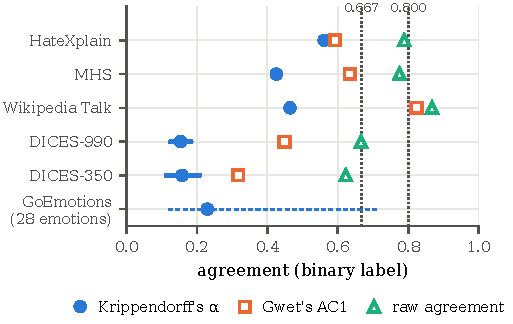
\includegraphics[width=\columnwidth]{figures/agreement.pdf}
\caption{Agreement on each corpus's binary label, with 95\% bootstrap intervals for $\alpha$ (most are narrower than the marker). For GoEmotions the dashed line spans the \nGoEmotions per-emotion values. Dotted lines: Krippendorff's 0.667 and 0.800.}
\label{fig:agreement}
\end{figure}
No corpus's main binary label reaches $\alpha=0.667$ (Figure~\ref{fig:agreement}). HateXplain is the most reliable at \alphaHx [\alphaLoHx, \alphaHiHx]; Wikipedia Talk (\alphaWiki) and MHS (\alphaMhs) follow; the DICES safety judgements are near \alphaDthree. GoEmotions varies by emotion from \alphaGoMin to \alphaGoMax (median \alphaGoMedian); only \goTopEmotion clears 0.667. So HateXplain's 3-way $\alpha$ of \alphaHxthree, which prompted this study, is not unusually low for its kind of task.

\paragraph{Coefficients disagree under skew.} On Wikipedia Talk, raw agreement is \rawWiki and AC1 is \acOneWiki, but $\alpha$ is \alphaWiki. Most comments are benign, so chance agreement is high and $\alpha$ discounts it; AC1 assumes lower chance agreement. The gap is a reminder that ``reliable enough'' must name its coefficient.

\paragraph{Subsampling matters for one corpus.} Keeping all ratings changes $\alpha$ by at most \allRatingsMaxShift on every corpus except MHS, where it rises from \alphaMhs to \alphaMhsAll: \mhsAnchorItems anchor comments rated by hundreds of people hold \mhsAnchorShare\% of all MHS ratings and dominate the coincidence matrix. We use the capped estimate.

\paragraph{Agreement bracket.} On HateXplain's binary label the agreement bracket runs from \ceilLooHx and \ceilInHx; \marginOneHx\% of items are decided by a single vote. On the official test split, \retroSplit\% of posts are 2--1 splits, and a held-out annotator matches the other two on \retroHuman\% of the posts where those two agree.

\section{Do claim gates make better decisions?}
\label{sec:gate}
We simulate binary truth, three raters with known error rates, and two systems with a known true accuracy gap and disagreement rate, and score both gates against the majority label of the simulated raters. The grid crosses prevalence, target $\alpha$ (0.2--0.9), test size (200--5,000), true gap ($-0.03$ to $0.05$) and system disagreement, with 1,000 replicates per cell (\simCellsIid cells). A \emph{false claim} is a published ``A beats B'' when the true gap is $\leq 0$; a claim is \emph{resolvable} when the true gap is $\geq 0.03$. Three further scenarios concentrate rater error on 30\% hard items: one, specified before any simulation result, puts the better system's advantage on the hard items; two, added after seeing results, put it on the clear items, mildly and strongly (Appendix~\ref{app:deviations}).

\begin{figure*}[t]
\centering
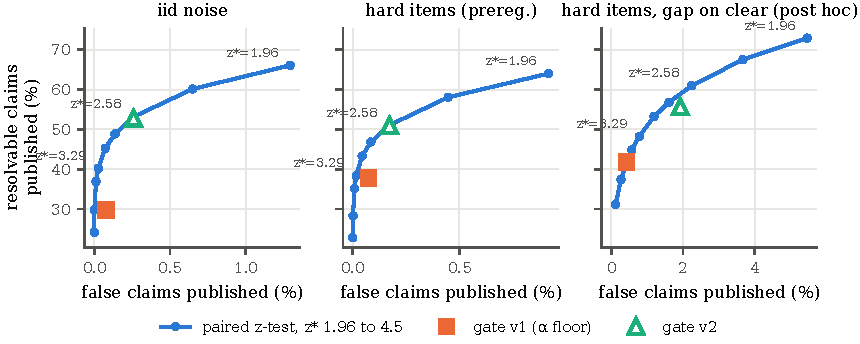
\includegraphics[width=\textwidth]{figures/gate_operating_points.pdf}
\caption{Share of false and resolvable claims each rule publishes. The line traces a plain paired $z$-test as its threshold rises from 1.96 to 4.5. Gate~v1 sits below the line: at its false-claim rate, a stricter $z$-test publishes more real differences. Gate~v2 sits on or just below the line: it is a $z$-test at 2.58 plus a contested-item check. The mild post-hoc scenario is reported in the text.}
\label{fig:gate}
\end{figure*}

\paragraph{The reliability floor buys fewer false claims at a higher power cost than a stricter test.} Under independent rater noise, gate~v1 publishes \simFalseVoneIid\% false claims and \simResVoneIid\% of resolvable ones; a plain $z$-test tuned to the same false-claim rate publishes \simResMatchedIid\% (Figure~\ref{fig:gate}). Part of this gap reflects the grid: \simShareLowAlphaCells\% of cells have target $\alpha<0.5$, where the floor blocks by design. Restricted to $\alpha\geq0.5$, gate~v1 publishes \simResVoneIidHi\% at a \simFalseVoneIidHi\% false-claim rate against \simResMatchedIidHi\% for the matched test, a smaller but consistent loss. The pattern holds when errors concentrate on hard items (\simResVoneHet\% vs.\ \simResMatchedHet\%) and in the mild post-hoc scenario (\simResVoneHetmild\% vs.\ \simResMatchedHetmild\%); only in the strong post-hoc scenario, built to favour the floor, do the two draw even (\simResVoneHetneg\% vs.\ \simResMatchedHetneg\%). Below $\alpha=0.5$ the floor blocks almost everything, publishing \simResVoneLowAlphaIid\% of resolvable claims where an ordinary test at 1.96 publishes \simResZlowLowAlphaIid\%. The reason is structural: for a binary label, gold noise does not manufacture a gap, it shrinks the real one, so a noisy benchmark calls for more items or a larger effect, not a veto. On real data the difference is starker: of the \jPairsTotal judge-versus-judge comparisons in \S\ref{sec:judges}, gate~v1 could publish only \jPairsVonePub, all on HateXplain, because every other corpus has $\alpha<0.5$.

\paragraph{Ablation.} Only two checks ever bind. Removing the $\alpha$ floor raises the resolvable publish rate from \ablResNone\% to \ablResRel\% and the false-claim rate from \simFalseVoneIid\% to \ablFalseRel\%, removing the MDE check raises it to \ablResMde\%, and removing any of the other three leaves it at \ablResCi\%. The pre-registered threshold sweep (Appendix~\ref{app:sweep}) shows the trade-off is monotone: every increase of the floor removes more real differences than false ones.

\paragraph{What gate~v2 adds.} Under independent noise gate~v2 matches a $z$-test at 2.58 (\simResVtwoIid\% resolvable, \simFalseVtwoIid\% false), so its blocking behaviour is essentially a significance test, and we present it as that. The contested-item check does not earn its place either: in the strong post-hoc scenario it blocks \simCthreeBlockShareHetneg\% of the claims that pass the $z$-test, lowering resolvable claims from \simResZmidHetneg\% to \simResVtwoHetneg\%, while a $z$-test at the same false-claim rate publishes \simResMatchedVtwoHetneg\%. We keep it as a diagnostic, not a safeguard. Gate~v2's value is the report: averaged over replicates, the attenuation estimate recovers the simulated $1-2\eta_k$ to within \attEstMaxErr at $n\geq1{,}000$.

\section{Could published gaps be resolved?}
\label{sec:retro}
\begin{figure}[t]
\centering
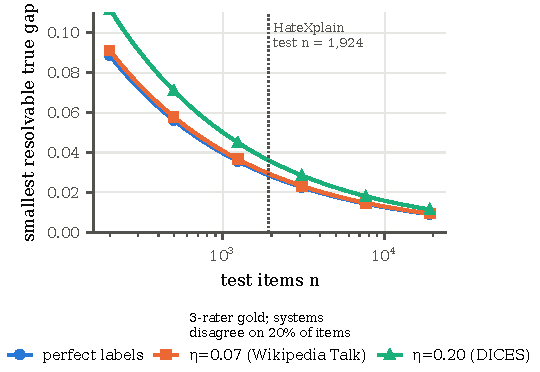
\includegraphics[width=\columnwidth]{figures/mde_vs_n.pdf}
\caption{Smallest true accuracy gap resolvable at 80\% power ($z^\ast=1.96$) by test size, for perfect labels and for three-rater gold labels at two single-rater error rates.}
\label{fig:mde}
\end{figure}
HateXplain reports six models' test accuracies \citep[Table 6]{mathew2021hatexplain}; its official test split has \retroN posts with a majority label. For each of the \retroPairs pairwise gaps we ask which system-disagreement rates would make it significant at $z=1.96$ (Appendix~\ref{app:retro}). Of these, \retroUnresolvable gaps, from \retroMinGap to \retroBertGap, are resolvable only if the two systems disagree on fewer than \retroMinPmax--\retroBertPmax\% of the test posts, implausible even for two training runs of one architecture. They include BERT-HateXplain vs.\ BERT and BiRNN-HateXplain vs.\ BiRNN-Attn, the comparisons that isolate the effect of rationale supervision on accuracy. Gaps of \retroAlwaysGap and above are resolvable at any disagreement rate. This does not bear on the paper's main claims, which concern bias and explainability, and published accuracies are rounded to three decimals. This analysis is about test size alone; gold-label noise only makes it worse, since the true gap must be $1/(1-2\eta_k)$ times larger than the observed one to be detected.

\section{Items or raters?}
\label{sec:k}
\begin{figure}[t]
\centering
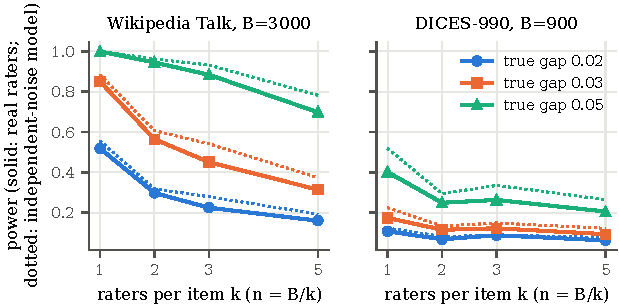
\includegraphics[width=\columnwidth]{figures/claim4_power.pdf}
\caption{Power to detect a true accuracy gap when a fixed budget $B$ is spent as $n=B/k$ items with $k$ real raters each. Dotted: prediction under independent rater noise.}
\label{fig:k}
\end{figure}
\citet{dorner2024dont} prove, for large enough budgets and assuming no biased heterogeneity, that a single label per item is optimal for identifying the better of two binary classifiers. We test this on real raters, whose errors are correlated and item-dependent. For every item with at least ten binary ratings (\clFourItemsWiki Wikipedia Talk comments, \clFourItemsDnine DICES-990 and \clFourItemsDthree DICES-350 conversations), we split raters into a pool of five and a disjoint reference panel whose majority serves as truth. Synthetic systems are drawn against the reference, either uniformly or with both systems erring more on contested items and the better system's advantage on clear items. A design spends budget $B$ on $B/k$ items rated by $k$ pool raters.

One rater per item gave the highest power in all \clFourCells cells (Figure~\ref{fig:k}), though in \clFourCellsClose of them the lead is within two Monte Carlo standard errors. With uniform systems, real raters made replication \emph{less} valuable than the independent-noise model predicts: observed power fell below the prediction in \clFourBelowUniform of \clFourRowsUniform designs with $k>1$ (e.g.\ \clFourWikiKthree vs.\ \clFourWikiKthreePred for $k=3$ on Wikipedia Talk, $B=6{,}000$, gap 0.03, against \clFourWikiKone for $k=1$). With contested systems the prediction was not systematically optimistic (\clFourBelowContested of \clFourRowsContested below). Wrong rankings were rarer with one rater per item (\clFourFlipKone\% of replicates on average) than with five (\clFourFlipKfive\%). This concerns accuracy against a majority reference; \citet{homan2026many} and \citet{pandita2026improving} show that distribution-sensitive metrics, or systems evaluated by several responses each, need more ratings per item, and measuring reliability at all needs a replicated subset.

\section{LLM judges against held-out humans}
\label{sec:judges}
We scored five judges (Claude Haiku~4.5, Claude Sonnet~5.5, GPT-4.1-mini, and the open-weight Qwen2.5 14B and gpt-oss 20B run locally) on fixed samples of up to 1,000 items per corpus (\jItemsTotal in total), with one pre-registered zero-shot prompt per corpus. For each item one annotator is held out; the remaining annotators form the panel. The held-out human and every judge are scored identically: agreement with the panel's binary majority on items where the panel has one. The human level, not 100\%, is the reference. Models, prompts, sample, parser and metrics were fixed before any call (Appendix~\ref{app:judges}); the API judges cost \$\jCostUsd.

\begin{figure*}[t]
\centering
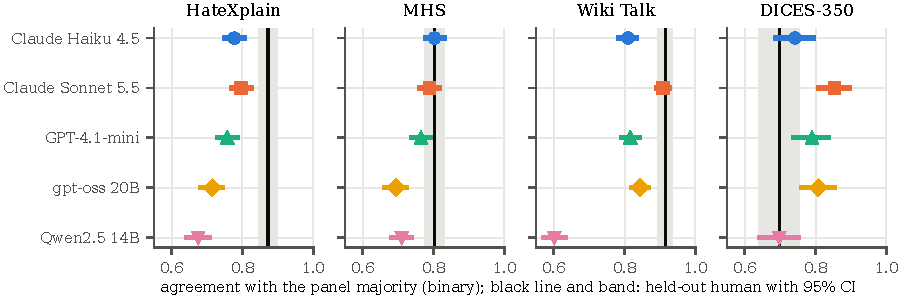
\includegraphics[width=\textwidth]{figures/judges.pdf}
\caption{Judge agreement with the panel majority (95\% bootstrap intervals). The black line and grey band mark a held-out human annotator scored on the same items.}
\label{fig:judges}
\end{figure*}

\begin{table*}[t]
\centering\small
\begin{tabular}{@{}lrrrrrrrr@{}}
\toprule
Judge & \multicolumn{2}{c}{HateXplain} & \multicolumn{2}{c}{MHS} & \multicolumn{2}{c}{Wiki Talk} & \multicolumn{2}{c}{DICES-350} \\
\midrule
Held-out human & 0.872 &  & 0.803 &  & 0.915 &  & 0.697 &  \\
Claude Haiku 4.5 & 0.777 & -0.095 & 0.803 & +0.000 & 0.810 & -0.105 & 0.742 & +0.044 \\
Claude Sonnet 5.5 & 0.796 & -0.077 & 0.788 & -0.015 & 0.908 & -0.006 & 0.853$^{\ast}$ & +0.147 \\
GPT-4.1-mini & 0.757 & -0.115 & 0.765 & -0.038 & 0.816 & -0.099 & 0.790$^{\ast}$ & +0.092 \\
Qwen2.5 14B & 0.675 & -0.198 & 0.710 & -0.093 & 0.601 & -0.314 & 0.697 & +0.000 \\
gpt-oss 20B & 0.715 & -0.158 & 0.694 & -0.109 & 0.844 & -0.071 & 0.808$^{\ast}$ & +0.111 \\
\bottomrule
\end{tabular}

\caption{Agreement with the panel majority and difference from the held-out human (judge $-$ human). $^\ast$Gate~v2 accepts ``judge beats the held-out human'' ($z>2.58$).}
\label{tab:judges}
\end{table*}

\paragraph{On the three toxicity and hate corpora, no judge beats a single human.} The best judge is at or below the held-out human on HateXplain (Sonnet \jSonnetHx vs.\ \jHumanHx), MHS (Haiku \jHaikuMhs vs.\ \jHumanMhs) and Wikipedia Talk (Sonnet \jSonnetWiki vs.\ \jHumanWiki; Table~\ref{tab:judges}, Figure~\ref{fig:judges}). Where the difference is small (Sonnet on Wikipedia Talk, \jDiffSonnetWiki [\jDiffLoSonnetWiki, \jDiffHiSonnetWiki]), the interval includes zero, so the honest statement is ``indistinguishable from one annotator'', not ``human-level''. The weakest judge, Qwen2.5 14B, is \jDiffQwenWiki below the human on Wikipedia Talk.

\paragraph{On DICES, three judges beat an individual rater, and this says more about the rater than the judges.} DICES has $\alpha\approx$ \alphaDthree, so a single rater is a weak reference: the held-out human reaches only \jHumanDthree. Sonnet (\jSonnetDthree), gpt-oss (\jOssDthree) and GPT-4.1-mini (\jGptDthree) exceed it, and gate~v2 accepts each claim. Against the dataset's expert safety labels, however, every judge (\jExpertQwen--\jExpertSonnet) is close to or below the held-out crowd rater (\jExpertHuman) and below the crowd panel's majority (\jExpertPanel). Beating a noisy individual is not the same as measuring the construct better.

\paragraph{The Sonnet result on DICES is fragile.} On \jSonnetDthreeUnparsed of 350 DICES conversations, Sonnet began explaining and reached its output limit before giving a label; no model refused any item (\jRefusals refusals in total), and no other judge--corpus pair had more than \jOtherInvalidMax unusable outputs. The pre-registered analysis excludes such outputs; scored as wrong, Sonnet's agreement falls from \jSonnetDthree to \jSonnetDthreeInvalidWrong, barely above the human. We did not re-run with a larger limit, because that would be a post-hoc change to a measured judge.

\paragraph{Alternative Annotator Test.} With the paper's default for crowd annotators ($\varepsilon=0.1$, Benjamini--Yekutieli at $q=0.05$), the test applies to HateXplain (\altAnnotHx annotators with at least 30 items) and DICES (\altAnnotDthree), and to neither MHS nor Wikipedia Talk, where no annotator has 30 items in the sample. No judge passes on HateXplain (winning rates \altQwenHx--\altHaikuHx, against the 0.5 required). On DICES four judges pass, Sonnet with a winning rate of \altSonnetDthree, consistent with the DICES result above. The test's requirement of dense annotation is itself a practical limit: most benchmarks cannot run it.

\paragraph{Comparing judges.} Gate~v2 resolves the direction of \jPairsPass of the \jPairsTotal judge-versus-judge comparisons; all \jPairsClose comparisons with gaps under 0.02 stay unresolved (\jPairsClosePass pass). A leaderboard of these judges built from the same samples could order the extremes but not the neighbours.


\section{Recommendations}
For a benchmark release: publish per-annotator labels and the test split; report $\alpha$ with an interval, AC1 and raw agreement together; report the agreement bracket and the one-vote share. For a comparison: report the paired disagreement rate and a paired test, and report the smallest true gap the test size and label noise can resolve. Do not replace a significance test with a reliability threshold; noisy labels call for larger test sets or larger effects. For LLM judges: compare with a held-out human on identical items and report both, since the human level, not 100\%, is the reference.

\ifdefined\PREPRINT
\section*{Code and data availability}
Code, results and paper sources: \url{https://github.com/yogvidwankhede/hatexplain-label-audit}, archived as \href{https://doi.org/10.5281/zenodo.23071900}{doi:10.5281/zenodo.23071900}. The statistics library: \url{https://github.com/yogvidwankhede/rubricon}, archived as \href{https://doi.org/10.5281/zenodo.23071898}{doi:10.5281/zenodo.23071898}. Corpora are downloaded from their original hosts by script; no corpus text is redistributed.
\fi

\section*{Limitations}
\textbf{Noise model.} The attenuation factor assumes binary labels, symmetric rater noise, and gold errors independent of the systems' errors. Real annotator disagreement is partly systematic \citep{davani2022dealing}; our hard-item scenarios and real-rater study probe this but do not cover every structure, and for multi-class labels we analyse only the binary collapse. \textbf{Simulation scope.} The gate comparison uses three raters and synthetic systems; the rankings of rules are stable across our scenarios, but other system-error structures could change them. Two of the four scenarios were added after seeing results and are labelled as such. \textbf{Pre-registration.} The plan was committed to version control and tagged before any new-corpus result was computed; the tag is a self-held git timestamp rather than a third-party registry, the tagged file still carries its draft header, and several analyses were added later (Appendix~\ref{app:deviations}). \textbf{Retrospective.} We use published, rounded accuracies without system outputs, so the analysis states conditions under which gaps are resolvable, not whether they were. It covers one paper. \textbf{Corpora.} All six corpora are English, and five concern toxicity, hate or safety, where disagreement is expected to be high; GoEmotions is the only non-harm task, and we found no NLI or sentiment corpus with rater identifiers and a clear licence. \textbf{Judges.} Judge prompts paraphrase the task definitions rather than reproduce the original guidelines; closed models change over time, and Claude Sonnet~5.5 does not accept temperature~0, and its output limit truncated \jSonnetDthreeUnparsed DICES answers before a label. Each judge was run once per item. \textbf{Alt-test.} It needs annotators with at least 30 items; in 1,000-item samples of MHS and Wikipedia Talk no annotator qualifies, so it applies only to HateXplain and DICES, and its HateXplain verdict depends on $\varepsilon$. We did not use its skew correction.

\section*{Ethics statement}
The hate-speech and abuse corpora contain offensive text about protected groups. We use them under their licences for research on measurement, quote no examples, and redistribute no text: the release contains code, item identifiers, labels and derived statistics, and each corpus is downloaded from its original host by a script. Worker identifiers are the corpora's own pseudonymous IDs; we do not attempt to link them to people, and GoEmotions user names are never read into results. Sending hateful text to commercial APIs exposes it to those providers; we excluded a provider whose free tier uses submitted content for product improvement. A risk of this work is that ``the labels cannot resolve this gap'' is misread as ``the result is wrong''; we state conditions, not verdicts, and name no result as erroneous.

\ifdefined\PREPRINT\section*{Acknowledgements}\else\section*{Use of AI assistants}\fi
\ifdefined\PREPRINT This work received no external funding. \fi In line with the ACL policy on AI writing assistance, we disclose that an AI coding assistant (Anthropic's Claude, via Claude Code) was used to write and test analysis code, run the experiments, search for and verify related work, and draft text, under the author's direction. The author reviewed the code, verified every citation against its source, and takes responsibility for all content. Separately, LLMs are \emph{objects of study} in \S\ref{sec:judges}; their use there is described in Appendix~\ref{app:judges}.

\bibliography{references}

\appendix
\section{Pre-registration and deviations}
\label{app:deviations}
The analysis plan (\texttt{PREREG.md}) was committed and tagged before any new-corpus statistic was computed. The HateXplain single-corpus results predate it and are replications. The judge addendum (\texttt{PREREG\_ADDENDUM.md}), fixing models, prompts, samples, the parser and the metrics, was committed before any model call; alt-test parameters were added before any alt-test result existed. Table~\ref{tab:dev} lists every departure; the repository's \texttt{DEVIATIONS.md} gives dates and whether results had been seen.

\begin{table*}[t]
\centering\small
\begin{tabular}{@{}p{0.2\textwidth}p{0.5\textwidth}p{0.22\textwidth}@{}}
\toprule
Change & What and why & Results seen before? \\
\midrule
Leave-one-out ceiling & Added a lower end to the ceiling bracket because the mean modal share includes the scored vote. & Only the already-published HateXplain value. \\
Separate seed & New analyses use a new master seed so the earlier HateXplain files still reproduce. & No. \\
Margin definition & Report exactly-one-vote lead and no-plurality separately. & HateXplain only. \\
Hard-item scenario (pre-registered model extended) & Added a second generative model with hard items; extended the gap grid to include negative gaps so false claims exist. & No. \\
Matched-threshold baseline & Compare gates with $z$-tests at matched false-claim rates. & Yes: aggregate gate rates. \\
Gate~v2 and two post-hoc scenarios & Designed after seeing that the $\alpha$ floor loses power; scenarios with the gap on clear items were added because the pre-registered scenario produced no extra false claims. & Yes. \\
Wider $z$ grid & Needed to reach gate~v1's false-claim rate in one scenario. & Yes. \\
Full-data bootstrap & Replaced the subsample bootstrap, whose interval excluded its own point estimate on one emotion. & Yes: first-run intervals. \\
Real-rater study details & Pool/reference split, system models and budgets fixed; one system model re-specified after an infeasibility crash, before any output. & No. \\
Judge pilot & DICES pilot items from DICES-990; a first-word parse rule added after pilot outputs began with a label and then explained. & Pilot only. \\
Sonnet sampling & Claude Sonnet~5.5 rejects temperature~0; default sampling used. & No. \\
\bottomrule
\end{tabular}
\caption{Departures from the pre-registered plan.}
\label{tab:dev}
\end{table*}

\section{All agreement statistics}
\label{app:cross}
\begin{table*}[t]
\centering\small
\begin{tabular}{@{}llrlrrlr@{}}
\toprule
Corpus & Label & $\alpha$ & 95\% CI & AC1 & Raw & Ceiling & $\alpha_{\text{all}}$ \\
\midrule
HateXplain & three way & 0.460 & [0.452, 0.467] & 0.469 & 0.644 & 0.644--0.814 & 0.460 \\
HateXplain & binary & 0.561 & [0.552, 0.571] & 0.592 & 0.789 & 0.789--0.894 & 0.561 \\
MHS & three way & 0.363 & [0.356, 0.370] & 0.585 & 0.686 & 0.695--0.835 & 0.470 \\
MHS & binary & 0.425 & [0.416, 0.434] & 0.634 & 0.775 & 0.781--0.883 & 0.537 \\
Wikipedia Talk & toxicity binary & 0.464 & [0.460, 0.469] & 0.823 & 0.867 & 0.895--0.924 & 0.466 \\
Wikipedia Talk & toxicity score & 0.296 & [0.293, 0.299] & -- & 0.482 & -- & 0.297 \\
DICES-350 & three way & 0.149 & [0.108, 0.190] & 0.400 & 0.556 & 0.613--0.729 & 0.161 \\
DICES-350 & binary & 0.158 & [0.113, 0.208] & 0.317 & 0.623 & 0.661--0.774 & 0.180 \\
DICES-990 & three way & 0.146 & [0.122, 0.172] & 0.482 & 0.602 & 0.659--0.759 & 0.143 \\
DICES-990 & binary & 0.154 & [0.124, 0.183] & 0.449 & 0.666 & 0.706--0.801 & 0.154 \\
\bottomrule
\end{tabular}

\caption{Agreement per corpus and label. Ceiling: leave-one-out to in-sample bracket. $\alpha_{\text{all}}$: all ratings kept instead of at most five per item.}
\end{table*}

\section{Threshold sweep}
\label{app:sweep}
\begin{figure}[h]
\centering
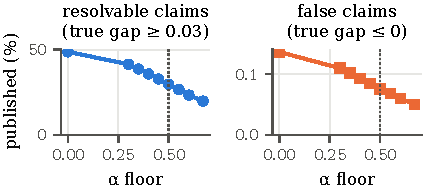
\includegraphics[width=\columnwidth]{figures/alpha_floor_sweep.pdf}
\caption{Gate~v1 under independent rater noise as its $\alpha$ floor varies (dotted: default).}
\end{figure}

\section{HateXplain gaps}
\label{app:retro}
For a paired comparison on $n$ items with discordance $p$ (the share of items exactly one system gets right), a gap $g$ has $z=g/\sqrt{(p-g^2)/n}$, so it is significant at threshold $z^\ast$ only if $p<p_{\max}=g^2(1+n/z^{\ast2})$. Since $p\geq g$, a $p_{\max}$ near $g$ means the gap cannot be resolved by any realistic pair of systems. Values are capped at 100\%.
\begin{table}[h]
\centering\small
\resizebox{\columnwidth}{!}{\begin{tabular}{@{}lrrr@{}}
\toprule
Comparison & Gap & $p_{\max}$ (\%), $z{=}1.96$ & $z{=}2.58$ \\
\midrule
BERT-HateXplain $>$ BiRNN & 0.103 & 100.0 & 100.0 \\
BERT $>$ BiRNN & 0.095 & 100.0 & 100.0 \\
BERT-HateXplain $>$ BiRNN-Attn & 0.077 & 100.0 & 100.0 \\
BERT-HateXplain $>$ CNN-GRU & 0.071 & 100.0 & 100.0 \\
BERT $>$ BiRNN-Attn & 0.069 & 100.0 & 100.0 \\
BERT-HateXplain $>$ BiRNN-HateXplain & 0.069 & 100.0 & 100.0 \\
BERT $>$ CNN-GRU & 0.063 & 100.0 & 100.0 \\
BERT $>$ BiRNN-HateXplain & 0.061 & 100.0 & 100.0 \\
BiRNN-HateXplain $>$ BiRNN & 0.034 & 58.0 & 33.5 \\
CNN-GRU $>$ BiRNN & 0.032 & 51.4 & 29.7 \\
BiRNN-Attn $>$ BiRNN & 0.026 & 33.9 & 19.6 \\
BiRNN-HateXplain $>$ BiRNN-Attn & 0.008 & 3.2 & 1.9 \\
BERT-HateXplain $>$ BERT & 0.008 & 3.2 & 1.9 \\
CNN-GRU $>$ BiRNN-Attn & 0.006 & 1.8 & 1.0 \\
BiRNN-HateXplain $>$ CNN-GRU & 0.002 & 0.2 & 0.1 \\
\bottomrule
\end{tabular}
}
\caption{Published HateXplain test-accuracy gaps and the largest disagreement rate at which each is resolvable.}
\end{table}

\section{Judge experiment details}
\label{app:judges}
\paragraph{Models.} Claude Haiku~4.5 (\texttt{claude-haiku-4-5-20251001}, temperature 0, 16 output tokens) and Claude Sonnet~5.5 (\texttt{claude-sonnet-5-5}, thinking off, effort low, 64 output tokens, default sampling because the model rejects temperature 0) through the Anthropic Message Batches API; GPT-4.1-mini (snapshot \texttt{gpt-4.1-mini-2025-04-14}, temperature 0, seed 0, 16 output tokens) through the OpenAI Chat Completions API; Qwen2.5 14B (\texttt{qwen2.5:14b}) and gpt-oss 20B (\texttt{gpt-oss:20b}, reasoning effort low) through Ollama on one Apple M4 Max, temperature 0, seed 0. No server-side fallback to another model was enabled. We excluded a free API tier whose terms state that submitted content is used to improve the provider's products, and a free tier whose daily token limit would have required more than a week.

\paragraph{Prompts.} One system prompt per corpus (the repository's \texttt{prompts/}, hashed in \texttt{PREREG\_ADDENDUM.md}), paraphrasing the corpus's question: HateXplain (hatespeech / offensive / normal), MHS (``Is this comment hate speech?'' yes / unclear / no), Wikipedia Talk (five-point toxicity scale, binarised at toxic), DICES (is the chatbot's final response unsafe: yes / no / unsure). The item text is the user message; there are no examples.

\paragraph{Sample and scoring.} Items with at least three ratings in the capped matrix; a seeded sample of 1,000 per corpus (all 350 for DICES-350); one seeded held-out rater per item. Outputs are parsed strictly (the answer is a label), then by first word, then leniently (exactly one label word); anything else is unusable. A formatting pilot on five items per corpus outside the sample led to the first-word rule; no evaluation output was seen before it was fixed.

\paragraph{Alternative Annotator Test.} Implemented from \citet{calderon2025alternative}: per annotator $j$, alignment $S(\cdot,x_i,j)$ is the mean agreement with the item's other annotators; win indicators $W^f=\mathbb{1}\{S_f\geq S_h\}$ and $W^h=\mathbb{1}\{S_h\geq S_f\}$; a one-sided $t$-test of $H_0{:}\ \rho^f_j\leq\rho^h_j-\varepsilon$ on $d=W^h-W^f$; Benjamini--Yekutieli across annotators; pass if the winning rate is at least 0.5. For DICES we use all ratings (123 raters per item), because the five-rating cap leaves no DICES rater with 30 items. We do not use the paper's skew correction.

\paragraph{Cost.} The three API judges used \$\jCostUsd at list prices (Batch API rates for Anthropic). Token counts per judge and corpus are in \texttt{results/judge/analysis.json}.



\end{document}
